
\documentclass{standalone}
\usepackage[svgnames]{xcolor}
\usepackage{pgfplots}
\pgfplotsset{compat=newest}
\usepackage[sfdefault]{FiraSans}
\usepackage{FiraMono}
\renewcommand*\familydefault{\sfdefault}
\begin{document}
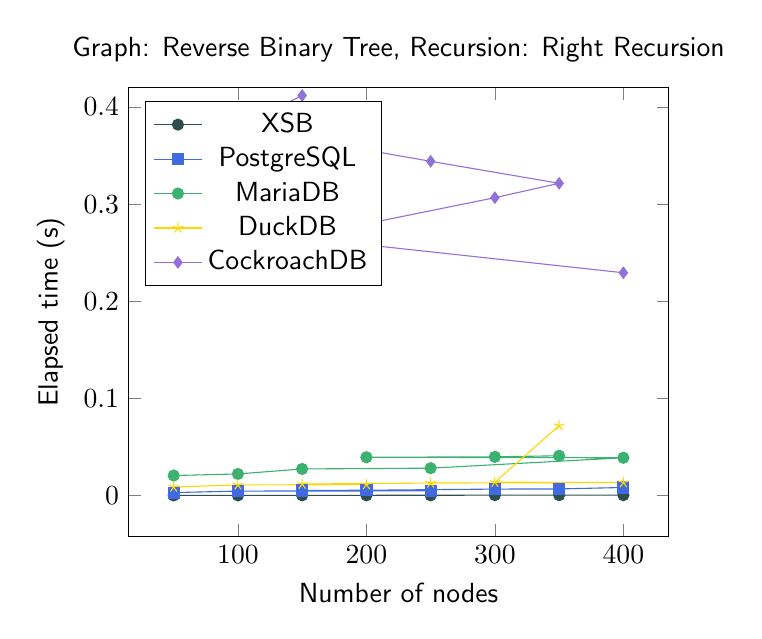
\begin{tikzpicture}
    \begin{axis}[
        title={Graph: Reverse Binary Tree, Recursion: Right Recursion},
        xlabel={Number of nodes},
        ylabel={Elapsed time (s)},
        legend pos={north west},
        ymax=0.41976059599983273
    ]
    \addplot+[DarkSlateGray, mark options={color=DarkSlateGray}] coordinates {(50,4.89950180053711e-05) (100,7.915496826171875e-05) (250,0.00015962123870849599) (150,0.000169038772583008) (200,0.0001795291900634765) (300,0.000338912010192871) (400,0.0003703832626342775) (350,0.0003905296325683595)};
\addlegendentry{XSB}
\addplot+[RoyalBlue, mark options={color=RoyalBlue}] coordinates {(50,0.00297904199999266) (100,0.004538243499951022) (250,0.004757548500037956) (150,0.005202022500043313) (200,0.005398761499918692) (300,0.006594999499952792) (350,0.0067403320000494205) (400,0.008252676499978406)};
\addlegendentry{PostgreSQL}
\addplot+[MediumSeaGreen, mark options={color=MediumSeaGreen}] coordinates {(50,0.02054970349990981) (100,0.02218251550016248) (150,0.027331713000194213) (250,0.028132825500051695) (400,0.03883957199991528) (200,0.03936372099997243) (300,0.039821547500196175) (350,0.040892266000128075)};
\addlegendentry{MariaDB}
\addplot+[Gold, mark options={color=Gold}] coordinates {(50,0.008744334500079276) (100,0.010870104499872468) (200,0.011213780000161933) (150,0.01179352100007236) (250,0.012807299499854707) (400,0.013344478999897547) (300,0.013668971000015517) (350,0.07194641299997784)};
\addlegendentry{DuckDB}
\addplot+[MediumPurple, mark options={color=MediumPurple}] coordinates {(400,0.22937174900016544) (50,0.2796714440000869) (200,0.2798230420000891) (300,0.3067002185000547) (350,0.32149513549984476) (250,0.34413536750003004) (100,0.3788926340000671) (150,0.4119600684998659)};
\addlegendentry{CockroachDB}

    \end{axis}
\end{tikzpicture}
\end{document}
